\chapter{Systeme}
\label{cha:systeme}
Die Entscheidungsgrundlage 
\section{Samsung Knox}


Ist man Besitzer aktueller Samsung-Geräten findet man die Applikation \textit{Sicherer Ordner}\footnote{Sicherer Ordner löste am 19. Dezember 2017 den Vorgänger MyKnox ab {sam2017b} }als vorinstallierte Standardsoftware vor. Mit Öffnen dieser App können, nach Eingabe eines benutzerdefinierten Sicherheitsverfahren, verschiedene Einstellungen getätigt werden. Es ist möglich Dateien oder Apps in diesen ""sicheren Ordner" zu verschieben. Sogar Apps die vorher nicht auf dem Smartphone vorhanden sind, können direkt vom Store geladen und installiert werden.Theoretisch wäre dieser Lösungsansatz genau richtig für die Verwendung von BYOD und zusätzlich sogar kostenlos. Dennoch wäre dies nicht umsetzbar im Enterprise-Umfeld.

Um den Anforderungen an eine BYOD-Lösung der Loco AG gerecht zu werden, benötigt es eine MDM-Möglichkeit. Dafür muss die IT-Administration die Möglichkeit haben die eingesetzten Geräte zu verwalten und somit an die firmeninternen Sicherheitsanforderungen anzupassen. Eine mögliche Lösung bietet Samsung mit der kostenpflichtigen Variante Samsung Knox Premium, die im Folgenden nach dem Kriterienkatalog belichtet werden soll.


Das Sicherheitsverfahren der Knox-Plattform aus fünf Komponenten \cite{sam2017}:
\begin{enumerate}
\item Mehrschichtige Sicherheit
\item Root-of-Trust
\item Secure Boot und Trusted Boot
\item TrustZone®
\item SE for Android
\end{enumerate}

\newpage


\section{MobileIron}

\subsection {Allgemein} 
Das Unternehmen MobileIron ist ein US-amerikanisches Unternehmen mit Hauptsitz in Kalifornien welches im Jahr 2007 gegründet wurde. MobileIron hat sich von Anfang an auf die Verwaltung von mobilen Endgeräten im Enterprise Umfeld spezialisiert. Das Unternhemen wurde 2017 im siebten Jahr in folge als Leader im Magic Quadrant von der Gartner Inc. neben VMWare, IBM und BlackBerry für MDM/EMM Suites gekürt. Das Softwareentwicklungsunternehmen bietet in Ihrem Produktportfolio verschiedene Bring Your Own Device Pakete mit zahlreichen Funktionen an. 
\subsection {Kompatibilität}
Der Hersteller MobileIron unterstützt in seinen Lösungen die  mobilen Endgeräte Apple iOS, Google Android und Microsofts Windows Phone. Zusätzlich können klassische Desktop Geräte mit den Betriebssystemen Microsoft Windows (ab 8.1) und Apple OS X (ab 10.9)  verwaltet werden. 
\subsection {Paketmodelle}
MobileIron bietet die drei verschiedenen Bundles „EMM Silver“, „EMM Gold“ oder „EMM Platinum“ seiner Bring Your Own Device Lösung an.
Das Basispaket „EMM Silver“ beinhaltet die Komponenten „Core“ „Sentry „und „Apps@Work“. Das Paket „EMM Gold“ ist um die Module „Email+“, „Docs@Work“ und „Web@Work“ erweitert. Durch die Wahl des Platinum Pakets ergänzt sich dieses wiederum um „Help@Work“, „Tunnel“, „MobileIron Monitor“ und „ServiceConnect-Integration“.

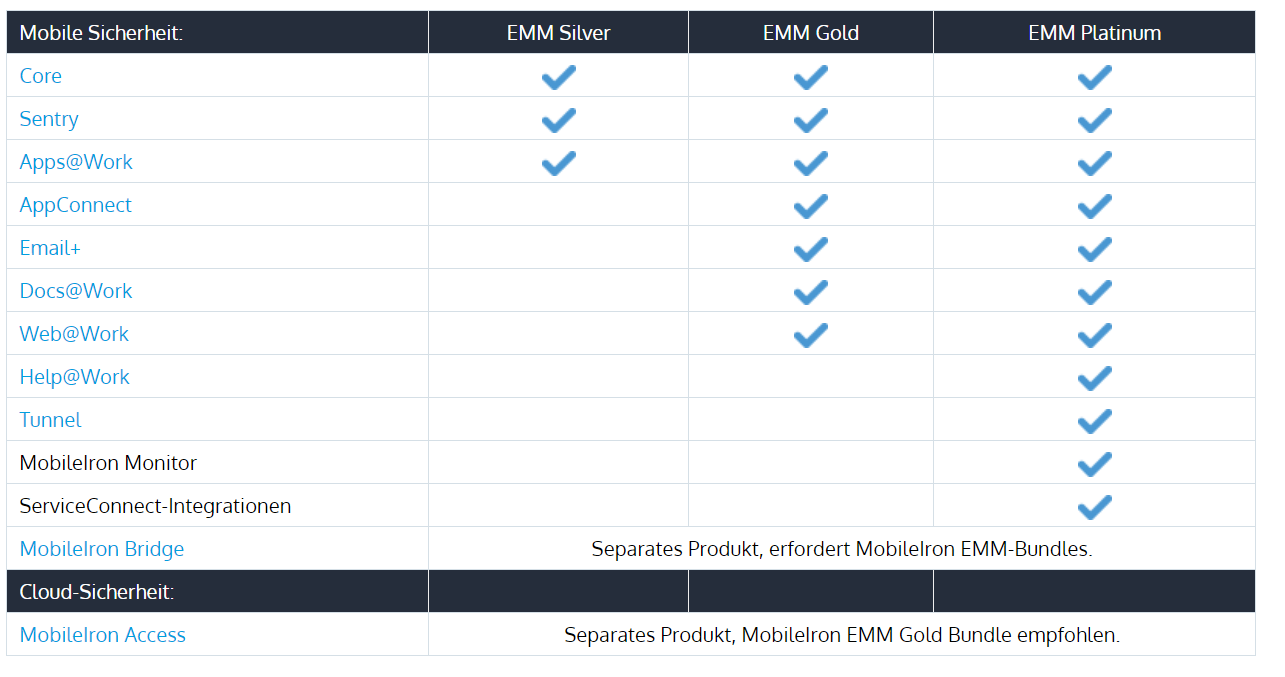
\includegraphics[width=0.95\textwidth]{Bilder/mi_1.png} 

\subsection {Pakete}
\subsubsection {Core}
Das Paket Core ist das zentrale Modul, welches das IT-Backend des Unternehmens einbindet. Hierüber können die erforderlichen Sicherheits- und Verwaltungsrichtlinien der mobilen Endgeräte definiert und verwaltet werden. Über die  API Schnittstellen des Cores kann man komfortabel Erweiterungen nutzen. Im Fokus des Cores stehen jedoch die das MDM, MAM und MCM. Der Core bietet für die Administratoren zusätzliche Analyse- und Auswerungsfunktionen. So kann beispielsweise der von den Endgeräten produzierten Netzwerktraffic ausgewertet werden um Infrastrukturprobleme zu lokalisieren. Durch die Möglichkeit Dachboards-Widgets anzulegen kann der Administrator das System und die verschiedenen Gerätestatus komfortabel überblicken. 
\subsubsection {Sentry}
Die Komponente Sentry ist das Inline-Gateway, das den gesamten Netzwerkverkehr zwischen den Mobilgeräten und dem Unternehmensbackend verschlüsselt, verwaltet und sichert. Sentry setzt die in der Core Komponente definierten Sicherheitsrichtlinien um. Sentry kann beispielsweise E-Mail Anhänge verschlüsseln, sodass nicht autorisierte Applikationen auf diese Daten nicht zugreifen können. 

\subsubsection {Apps@Work}
Apps@Work ist ein unternhemenseigener App Store, indem sowohl eigenentwickelte als auch öffentliche, freigegebene Anwendungen für die Benutzer bereitgestellt werden können. Über diesen Weg können Administratoren schnell auswählen, welche Anwendungen erforderlich, zulässig oder verboten sind. 
\subsubsection {AppConnect}
Durch AppConnect können auf den Endgeräten installierte Applikationen geschützt werden. Hierbei werden die entsprechenden Anwendungen in Containern gekapselt und sind somit vor unberechtigtem Zugriff geschützt. Alle in Containern befindlichen Apps können durch eine Tunnellösung miteinander kommunizieren um beispielsweise die Funktion eines Single Sign Ons bereitzustellen oder den Austausch von Daten bereitzustellen. 
\subsubsection {Email+}
Die gesamte Unternehmenskommunikation über mobile Endgeräte kann über die App Email+ abgewickelt werden. Die Anwendung stellt E-Mails, Kalender und Kontakte dar. Dabei findet eine strikte Trennung von beruflichen und privaten Inhalten statt. 
\subsubsection {Docs@Work}
Die Anwendung Docs@Work ist ein Tool um Dokumente auf Endgeräten zu verwalten und zu editieren. Hierbei ist ein besonderes Augenmerk auf die Synchronisation und Sicherung der Daten gelegt. 
\subsubsection {Web@Work}
Der Unternehmensbrowser Web@Works bietet dem Benutzer die Möglichkeit auf intern betriebene Webseiten oder Webapplikationen zuzugreifen.  Dabei ist die komplette Kommunikation verschlüsselt. Über verschiedene Benutzergruppen können die  Zugriffsrechte  auf die verschiedenen internen Webressourcen reglementiert werden. 
\subsubsection {Help@Work}
Help@Work ist ein Tool für die Fehlerdiagnose. Neben dem Abfragen und Übertragen von Ereignisprotokollen kann unter dem Betriebssystem Android sogar ein Remotezugriff für den IT-Support gewährt werden. 
\subsubsection {Tunnel}
Der Tunnel von MobileIron bietet die Möglichkeit die Netzwerkkommunikationen einzelner Apps durch eine VPN Verbindung auf der Basis von Zertifikaten zu schützen.

\subsection {Abrechnungsmodell}

Je nach Tarifplänen bzw. Paketangeboten werden neben den genannten Grundfunktionen weitere Features unterstützt. Das Unternehmen selbst betreibt ein sehr flexibles Abrechnungsmodell, welches auf jegliche Bedürfnisse des Endkunden angepasst werden kann. Dabei kann beispielsweise zwischen einer Lizenzierung pro Benutzer (maximal 3 Endgeräte) oder einem Lizenzierungsmodell je nach Endgerät gewählt werden. Neben der Kaufoption von Lizenzen auf Lebenszeit wird auch ein Abonnement angeboten. Neben der klassischen Installation innerhalb des eigenen Netzwerks betreibt MobileIron auch eine eigene Cloud die für die Bereitstellung der Services genutzt werden kann. Falls sich der Endkunde für die Cloudlösung entscheidet kann direkt ein erweiterter Support (SLA) dazu gebucht werden. Für die Installation auf einem eigenen System kann hierbei nur zwischen einem Standard- und Premiumsupport unterschieden werden.  

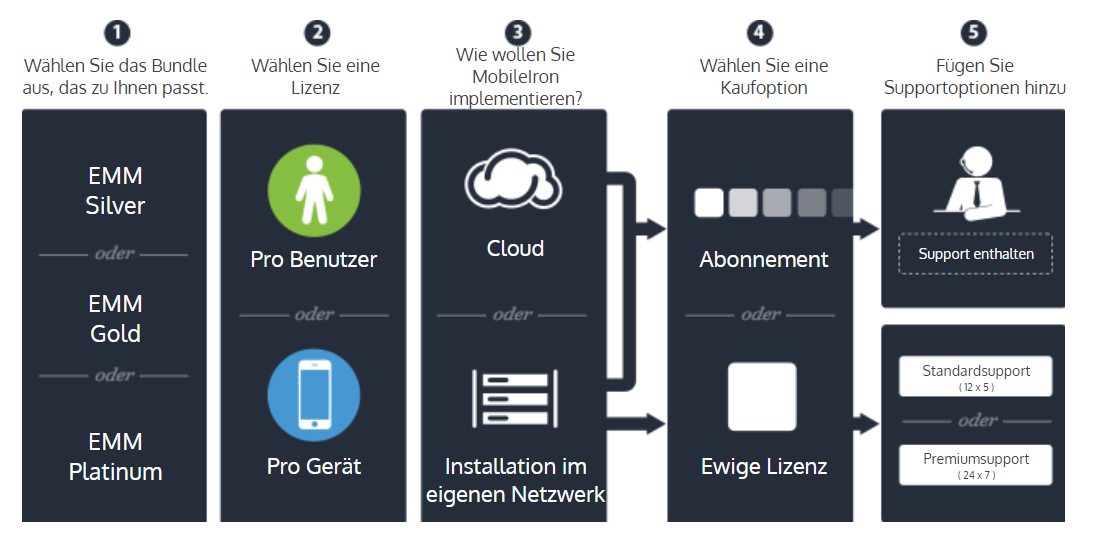
\includegraphics[width=0.95\textwidth]{Bilder/mi_2.png} 